% !TEX program = xelatex
\documentclass[blue,normal,cn]{elegantbook}

\usepackage{pdflscape}

\title{Sirius 设计文档}
\version{0.01}
\date{\today}

\begin{document}

\tableofcontents
\mainmatter

\chapter{设计概述}

比赛的核心要求是实现一个部分兼容 MIPS32 体系结构的小端序 CPU,并在其基础上搭建 SoC。
为了保证系统的简洁性,我们的 CPU 实现了最常用的部分 MIPS32 指令以及运行操作系统
等高级应用所必须的协处理器 CP0 等特权资源。

我们实现的处理器命名为 Sirius,采用了\textbf{双发射}五级流水线的设计,并支持一级指令、数据
缓存,以提升系统性能。一级缓存目前采用直接映射的方式,行宽 64 字节,大小为 8 KB。

通过运行功能测试以及性能测试,我们一定程度上证明了该处理器的正确性。

\section{指令系统}

根据大赛要求,我们实现的指令系统为 MIPS32 指令系统的子集,准确的说,我们
实现的指令系统包含全部 MIPS I 中的非浮点部分以及 MIPS32 中为了实现从异常
返回而添加的 ERET 指令。该指令系统包含以下几种指令类型:

\begin{itemize}
    \item \textbf{算数运算指令}\ 包括 ADD、SUB、SLT、MULT、DIV 等指令
    \item \textbf{逻辑运算指令}\ 包括 AND、OR、XOR、NOR、LUI 等指令
    \item \textbf{移位运算指令}\ 包括 SLL、SRL、SRA、SLLV、SRAV 等指令
    \item \textbf{分支跳转指令}\ 包括 J、JR、JAL、B、BEQ 等指令
    \item \textbf{内存访问指令}\ 包括 LB、LH、LW、SB、SW 等指令
    \item \textbf{系统控制指令}\ 包括 SYSCALL、BREAK、MFC0、MTC0 等指令
\end{itemize}

大赛文档给出的 57 条指令,我们均已正常实现。CPU 中包含的 32 个通用寄存器,HI、LO寄存器,
以及协处理器(CP0) 中实现的寄存器均按照 MIPS32r1 的规范实现。

基于性能方面的考虑,我们的 CPU 实现为非对称双发射五级流水线,通过对数据通路
和控制模块的精心设计,我们尽可能地解决了因数据冲突、控制冲突以及结构冲突导致
的流水线暂停。在我们的设计中,MIPS 传统的延迟槽技术得以保留,任一分支跳转
指令后面均有深度为一条指令的延迟槽,可以用于编译器优化。

\section{内存管理}

处理器的 MMU(内存管理)模块负责将虚地址映射为对应的物理地址,我们的 CPU 目前
只实现了 MIPS32r1 规范中规定的 kseg0 以及 kseg1 两段内存地址的映射,这两部分
的映射方式很简单。仅仅将物理地址的高三位置为 0 即可。后续的版本会实现完整的内存
地址映射。

\section{缓存}

在实际系统中,访存带宽与处理器运算能力的不匹配,使得访存系统的性能成为
了处理器系统性能的瓶颈。考虑到缓存能够直接减少微处理器与慢速的内存设备
之间的差距。我们的设计引入了缓存模块,用于进一步提升处理器的性能。

我们实现的 L1 Cache 共分为两部分:L1 指令缓存以及 L1 数据缓存。两者配置
完全相同,大小为 8 KB,行宽 64 字节,采用直接映射的方式进行替换。当命中时
L1 Cache 可以在单周期内返回数据,否则就会暂停流水线与内存设备进行交互。
L1 Cache 与 MMU 结合在一起,对外采用 AXI 接口,支持猝发(Burst)传输,
一次传输请求可以处理一整行缓存数据,以此提高总线的利用率。

\section{异常处理}

为了支撑操作系统的运行,提高处理器的通用性,Sirius 支持异常处理。根据 MIPS 
规范的要求,Sirius 支持精确异常。即 CPU 能准确记录发生异常的指令位置
(包括位于延迟槽中的指令),并确保异常发生之前的指令均完全执行,且让发生异常
的指令及之后的指令取消执行。按照优先级排序,我们的 CPU 支持如下异常:

\begin{enumerate}
    \item \textbf{中断}\ 外部中断、软中断、计时器中断。是否触发中断
    由协处理器0中的 Cause.IP 和 Status.IM 两个字段共同决定。
    \item \textbf{地址错例外:取指}\ 在取址阶段地址不对齐时触发该异常。
    \item \textbf{保留指令例外}\ 在解码阶段发现该指令无法解码时触发该异常。
    \item \textbf{自陷、系统调用}\ 当执行了对应的指令时触发这些异常。
    \item \textbf{整形溢出}\ 当执行 ADD、SUB、ADDI、SUBI 时发生溢出时触发该异常。
    \item \textbf{地址错例外:访存}\ 在访存阶段地址不对齐时触发该异常。
\end{enumerate}

异常发生后,PC 会被置为 0xBFC00380,开始异常处理流程。对于已经实现的异常,其处理流程
遵循比赛要求的处理流程。中断会受到 CP0 寄存器的影响。Sirius 支持 6 个硬件中断,它们分别由 CP0 
中的 Status.IM7 至 Status.IM2 位控制,对应位为 1 时中断启用。软中断则
由 Status.IM1 和 Status.IM0 控制。中断仅在处理器正常状态下才可以发生。

\section{CP0}

CP0 本质上为一组寄存器。Sirius 实现了大赛文档要求的全部 CP0 寄存器。同时
为了支撑后续的操作系统实现,我们拟额外实现一些 MIPS32r1 规范中要求的寄存器。
详见附录。

\chapter{Sirius CPU}

\section{总体设计}

Sirius CPU 设计为双发射五级流水线,分为取指、解码、执行、访存以及写回五个
流水级。在取指阶段,PC 中的值被送往 MMU,并在 MMU 被翻译为对应的物理地址,
并被送往 MMU 中取指相关的部分。如果该虚地址所在的区域可以被缓存,MMU 会先
在内置的 L1 指令缓存内查询该指令。如果缓存命中则在单周期内返回指令数据,否则
会发起访存请求充填流水线并暂停处理器。如果虚地址所在的区域不可被缓存,则直接
发起访存请求并暂停流水线直到数据返回。取到的指令以及与之对应的 PC 地址会被送到
指令 FIFO 内等待被执行。在译码阶段,指令 FIFO 的前两条指令会被取出,并被
翻译为处理器内部使用的指令。最后双发射判断逻辑会根据情况来决定是否发射第二条
指令,同时指令 FIFO 会根据双发射判断逻辑的结果确定是否删除刚刚被取出的两条
指令。在执行阶段,最多两条指令会并行地在两个 ALU 内执行。同时在执行阶段,分支
跳转等指令也在此执行,一旦确定需要跳转,需要跳转到的地址会被送回到 PC,PC 会在
下一周期更新到目的地址。执行阶段产生的结果会被送往访存阶段,在访存阶段首先会
处理异常,一旦有异常发生则刷新流水线。如果没有任何异常产生则正常进行访存操作。
访存操作会将数据以及地址等控制信息发送到 MMU 内,MMU 依然负责虚拟地址转换,
L1 数据缓存查找等操作。访存阶段的结果会被送到写回阶段。在写回阶段,运算/访存
结果被写入寄存器中。

为了处理数据冲突问题,我们的处理器引入了旁路机制,各个阶段的运行结果都会被前推
到解码阶段。当通过前推无法解决数据冲突时(如 load-use 冲突),流水线会暂停一拍
等待结果返回。对于跳转指令导致的控制冲突,我们使用 MIPS 的延迟槽机制尽可能的
使流水线不中断。在后续还将考虑引入分支预测器以及循环缓冲区进一步保证指令流不被
打断。

为了遵循 MIPS32r1 的规范,Sirius CPU 实现了精确异常处理。其实现方法是当异常
发生时,不直接处理,而是将之保存在流水线的寄存器内,直到访存阶段时统一处理。一旦
发生异常,则刷新流水线更新 PC。

\begin{landscape}\centering
    \vspace*{\fill}
    \begin{figure}[htpb]
        \centering
        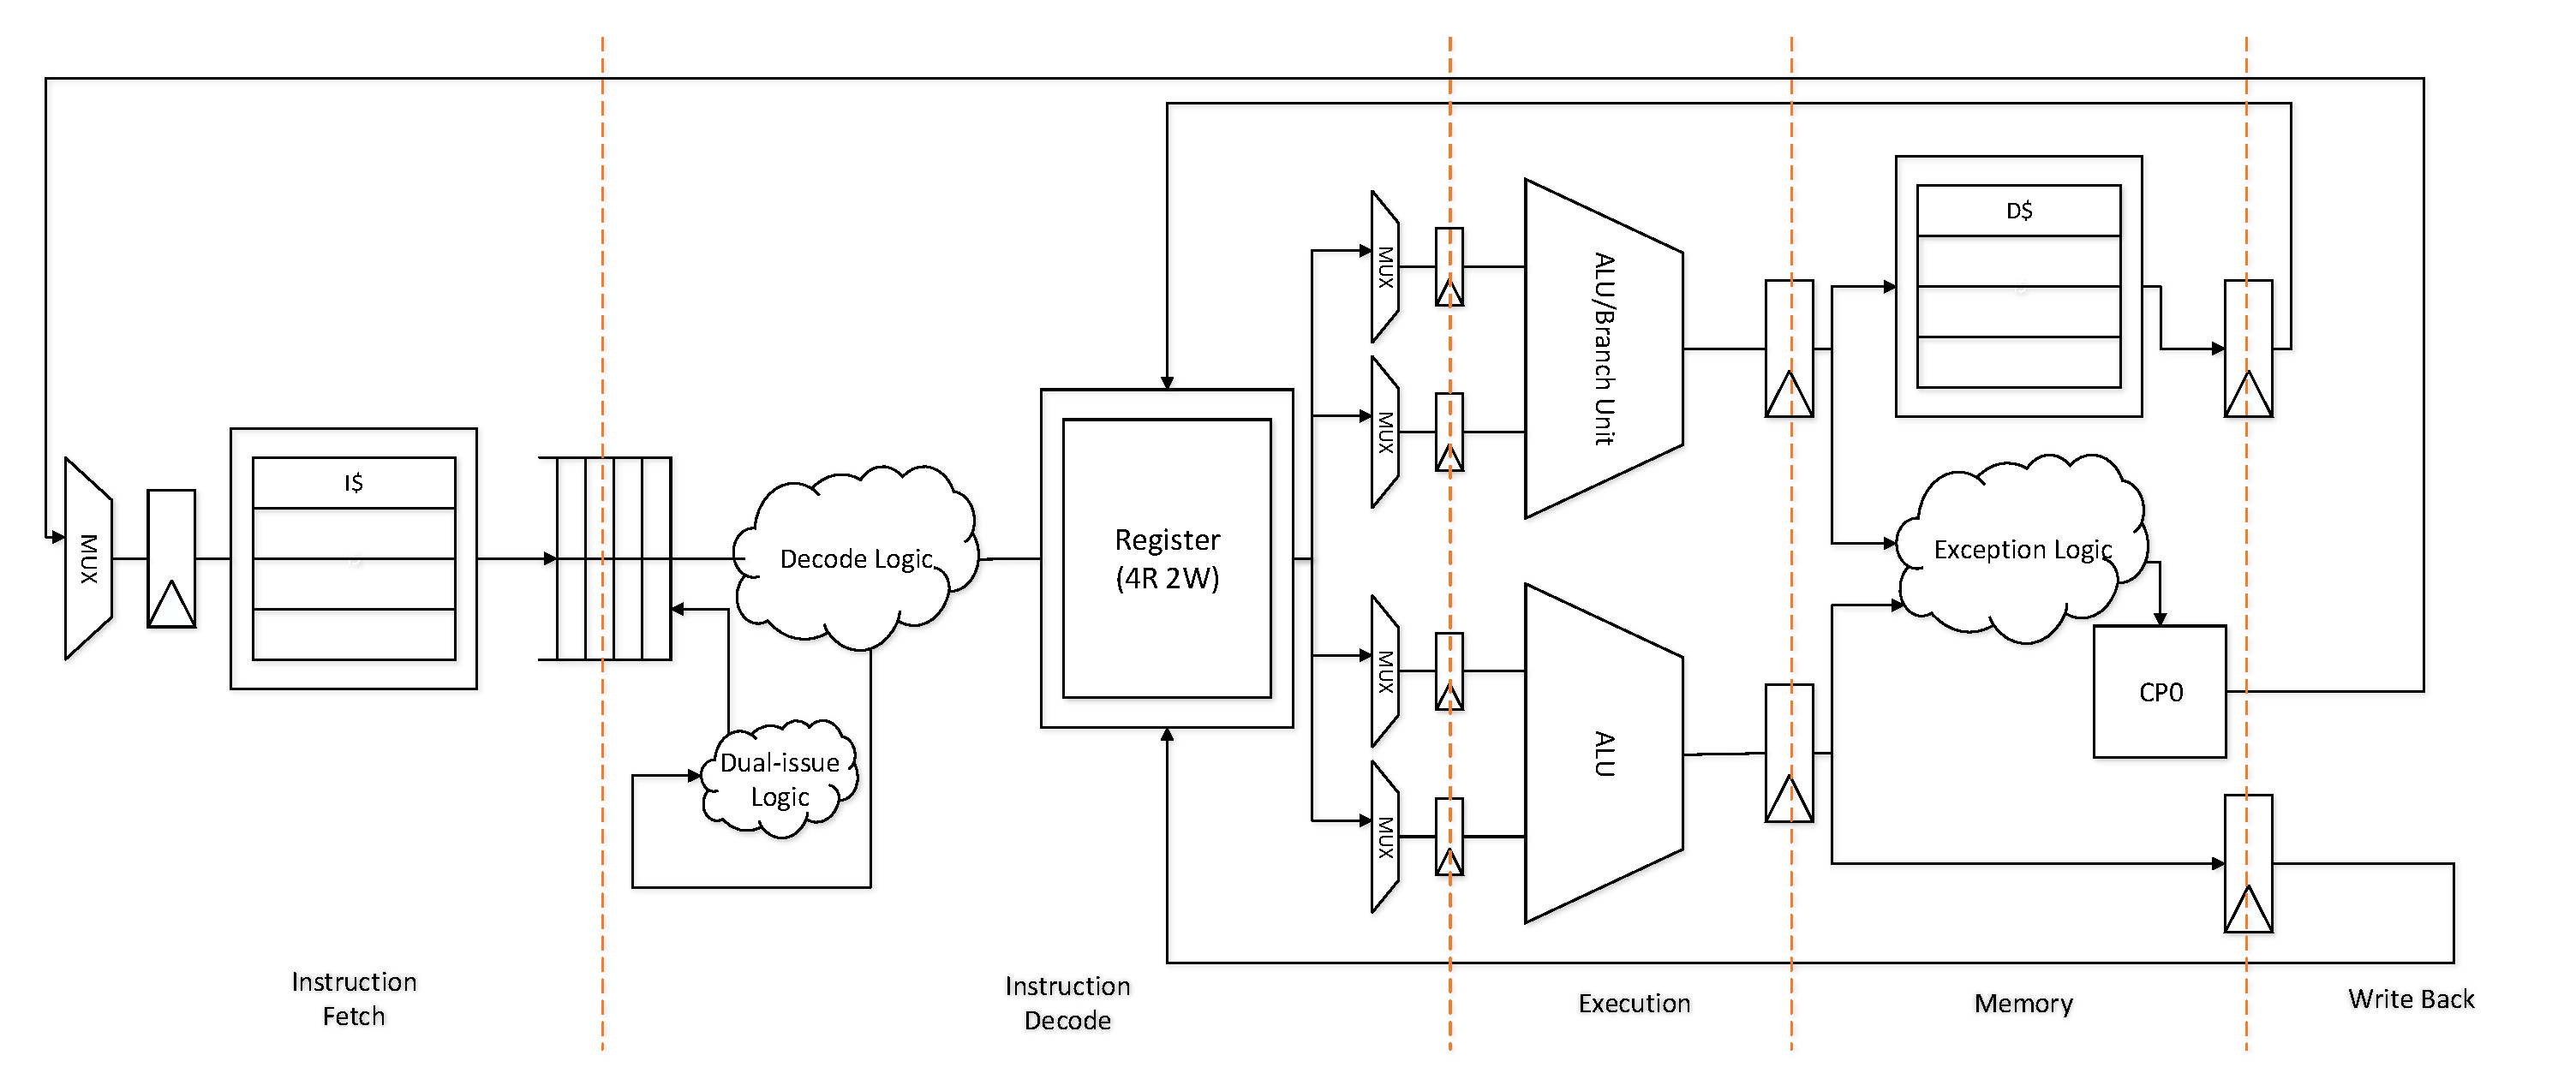
\includegraphics[width=1.65\textwidth]{figures/Sirius.pdf}
        \caption{Sirius 流水线设计}
        \label{fig:Test}
    \end{figure}
    \vfill
\end{landscape}

\end{document}